% https://tex.stackexchange.com/a/433812
\documentclass[xcolor={dvipsnames,table}, fleqn]{beamer}
\usefonttheme{professionalfonts}

\usepackage{tikz}
\usepackage{pgfplots}
\usepgfplotslibrary{colorbrewer}

\pgfplotsset{
    % initialize Dark2
    cycle list/Set2,
    % combine it with 'mark list*':
    cycle multiindex* list={
        mark list*\nextlist
        Set2\nextlist
    },
}


\begin{document}

\begin{frame}[fragile]

\begin{figure}
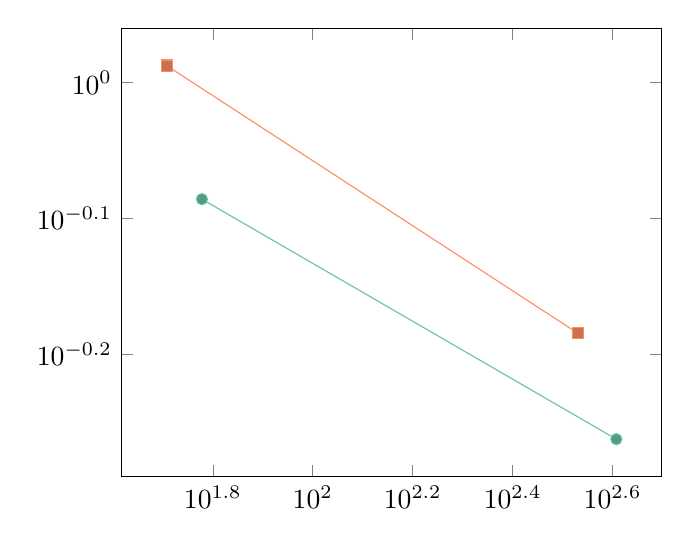
\begin{tikzpicture}
    \begin{loglogaxis}

\addplot + table[row sep=crcr]{%
60          0.8209744486252566 \\
405         0.5465621514772466\\
};
\addplot + table[row sep=crcr]{%
51          1.0295914003166593\\
339          0.6542156171940078 \\
};

   \end{loglogaxis}

\end{tikzpicture}
\end{figure}


\end{frame}

\pgfplotsset{cycle list shift=2}


\begin{frame}[fragile]

\begin{figure}
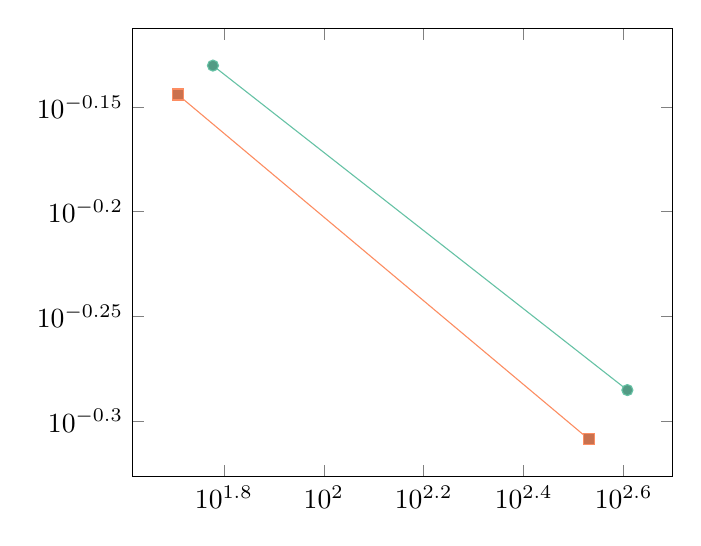
\begin{tikzpicture}
    \begin{loglogaxis}

\addplot table[row sep=crcr]{%
60          0.7412105340227999 \\
405         0.5183949403933881\\
};
\addplot table[row sep=crcr]{%
51           0.7179052621980517 \\
339          0.4911184551364445 \\
};

   \end{loglogaxis}

\end{tikzpicture}
\end{figure}

\end{frame}

\end{document}
